\chapter{Appendices}

\section[Responsabilités sur le site]{Responsabilités sur le site (juillet 2023)}\label{sec:responsabilitesSite}

L'appartenance à une catégorie implique l'appartenance à la catégorie suivante.

\subsec{Compte <<~User One~>>}

La notion de <<~User One~>> et propre à \emph{Drupal}, l'outil avec lequel sont créés les sites \CF. Ces comptes sont les seuls à avoir le droit de tout faire sur le site.

\begin{itemize}
    \item Laurence \textsc{Dumas}\footnote{Laurence Dumas est dans l'équipe de \CF, c'est elle qui a créé notre site mais elle n'appartient pas au \CdS.}
\end{itemize}

\subsec{Comptes SEL}\label{sec:comptesSel}

Il n'y a pas (que je sache) de prérogatives particulières attachées aux Comptes SEL

\begin{itemize}
    \item Laurence \textsc{Dumas}
    \item Camille-Aimé \textsc{Possamaï}
\end{itemize}

\subsec{Administrateur local}\label{sec:adminLocal}

Les administrateurs locaux peuvent effectuer certaines opérations sensibles sur le site, notamment gérer les membres (ajout, suppression, modification de statut, etc.).

\begin{itemize}
    \item Laurence \textsc{Dumas}
    \item Mathieu \textsc{Pellegrin}
    \item Camille-Aimé \textsc{Possamaï}
\end{itemize}

\subsec{Comité}\label{sec:comite}

Les membres du Comité peuvent, notamment, diffuser des actualités, enregister des documents.

\begin{itemize}
    \item Laurence \textsc{Dumas}
    \item Jacqueline \textsc{Lelong}
    \item Jackson \text{Michel}
    \item Mathieu \textsc{Pellegrin}
    \item Camille-Aimé \textsc{Possamaï}
\end{itemize}

\section{Profil complet de Charlotte}

De nombreuses captures d'écran de ce document ont été prises alors que le profil de Charlotte n'était pas complet. Il comportait seulement les informations indispensables pour créer un compte \CF, un prénom et une adresse courriel (celle qu'on voit sur certaines figures \texttt{charlotte.arnaud2@monfai.xyz} est fantaisiste). À la page suivante, vous trouverez son profil correctement rempli.

\begin{figure}
    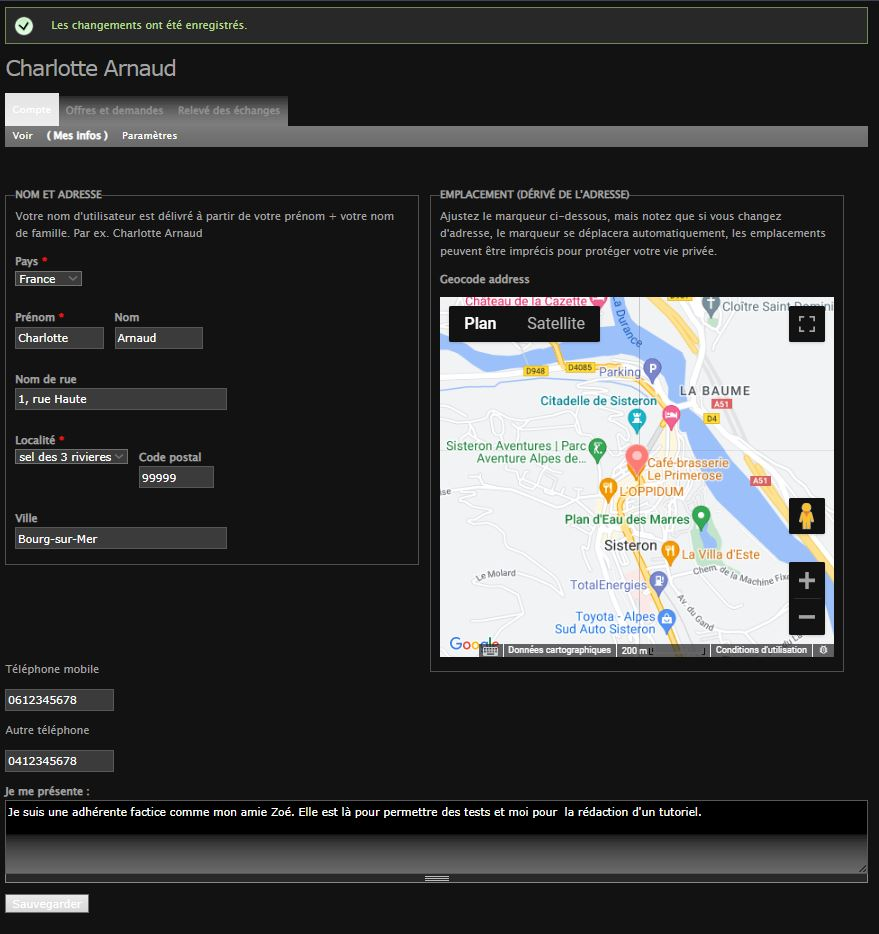
\includegraphics[width=\linewidth]{300-profil_charlotte_complet}
    \caption[Profil complet de Charlotte \textsc{Arnaud}]{Profil complété, onglet <<~Mes infos~>>, de Charlotte \textsc{Arnaud} notre adhérente factice  (l'adresse de Bourg-sur-Mer étant fantaisiste, le positionnement sur la carte est resté à Sisteron !)}
    \label{fig:profil_charlotte_complet}
\end{figure}

% \newpage

% \section{Nouveaux documents}